\documentclass[11pt]{beamer}
\usetheme{Madrid}
\usepackage[utf8]{inputenc}
\usepackage{amsmath}
\usepackage{amsfonts}
\usepackage{amssymb}
\usepackage{graphicx}
\usepackage{amsrefs}
\usepackage{algorithm}
\usepackage{algorithmic}
\usepackage{bbm}
\usepackage{subfigure}


\DeclareMathOperator {\argmin}{argmin}

\author{Hongda Li}
\title{Metropolis Hasting Chain and Simulated Annealing}
% Informe o seu email de contato no comando a seguir
% Por exemplo, alcebiades.col@ufes.br
\newcommand{\email}{email}
%\setbeamercovered{transparent}
\setbeamertemplate{navigation symbols}{}
%\logo{}
\institute[]{UBC Okanagan}
\date{\today}
%\subject{}

% ---------------------------------------------------------
% Selecione um estilo de referência
\bibliographystyle{plain}

%\bibliographystyle{abbrv}
%\setbeamertemplate{bibliography item}{\insertbiblabel}
% ---------------------------------------------------------

% ---------------------------------------------------------

\begin{document}

\begin{frame}
    \titlepage
\end{frame}

\begin{frame}{ToC}
    \tableofcontents
\end{frame}

\section{Introduction}

    \begin{frame}{The MHC}
        \begin{block}{MHC: Metropolis Hasting Chain}
            \begin{algorithmic}[H]
                \STATE{\textbf{Input: $X^{(t)}$}}
                \STATE{$Y^{(t)} \sim q (\cdot | x^{(t)})$}
                \STATE{
                    $ 
                    \rho(x, y) := 
                    \min\left\lbrace
                        \frac{f(y)}{f(x)}\frac{q(x|y)}{q(y|x)}, 1
                    \right\rbrace
                    $ 
                }
                \STATE{
                    $
                    X^{(t + 1)} := 
                    \begin{cases}
                        Y^{(t)} & \text{w.p}:  \rho(X^{(t)}, Y^{(t)})
                        \\
                        X^{(t)} &  \text{else}
                    \end{cases}$
                }
            \end{algorithmic}
        \end{block}
        \begin{itemize}
            \item [1.] $q(x|y)$ is doubly stochastic. 
            \item [2.] $f(x)$ is a distribution function up to a constant. 
            \item [3.] Must have $f(X^{(t)}) > 0$. 
        \end{itemize}
    \end{frame}
    \begin{frame}{What it does}
        Let $X^{(t)}$ be a sequence of observations sampled from the MHC, then $X^{(t)}$ will approximate $f$. 
        \begin{itemize}
            \item [1.] No integrals are needed. 
            \item [2.] It works very well for distribution functions in a very high dimension. 
            \item [3.] It is not hard to implement it on a computer. 
        \end{itemize}
    \end{frame}
    \begin{frame}{Primary questions}
        We have questions: 
        \begin{itemize}
            \item Is $f$ a stationary distribution for the MHC? 
                \begin{itemize}
                    \item Yes. 
                \end{itemize}
            \item Does it converge to the stationary distributions $f$? 
            \begin{itemize}
                \item Sometimes. We need some regularity conditions. 
            \end{itemize}
        \end{itemize}
        \vspace{2em}
        To converge to $f$ the MHC must satisfy the following: 
        \begin{itemize}
            \item [1.] $f$ is a stationary distribution of the MHC. 
            \item [2.] All states in $\text{supp}(f)$ can be commuted with each other. (f-Irreducible)
            \item [3.] All states are aperiodic. 
        \end{itemize}
    \end{frame}
    \begin{frame}{The transition kernel}
        \begin{block}{The transition kernel for MHC}
            \begin{align*}
                K(x, y) = 
                \rho(x, y)q(y|x) + 
                \left(
                    1 - \underbrace{\sum_{z \in S\setminus \{y\} }^{}\rho(x, z)q(z|x)}_{=:r(x)}
                \right) \mathbbm 1\{y = x\}. 
            \end{align*}
        \end{block}
        \begin{itemize}
            \item [1.] When $q$ is doubly stochastic, $f$ satisfies detail balance. ($f$-stationary)
            \item [2.] We have $K(x,x)> 0$ for all $x$ such that $f(x) > 0$. It is aperiodic. 
            \item [3.] It is f-irreducible if we assume $q(x|y)$ is non-negative for all $x, y\in \text{supp}(f)$. 
            \item [4.] See Robert and Casella's book \cite{book:robert_casella_2005} for the case where state space is continuous. 
        \end{itemize}
    \end{frame}
    \begin{frame}{Regularity conditions}
        \begin{itemize}
            \item [1.] $X^{(t)}$ needs to be able to travel to all states in $x\in \text{supp}(f)$. 
            \item [2.] And this is possible if $q(x|y) > 0 \;\forall x, y\in S$. 
            \item [3.] Weaker conditions exist, and we might have to do that in a case-by-case basis. We need to have: 
        \end{itemize}
        \begin{align*}
           \forall x,y \in S\times S \;\exists n < \infty: K^n(x, y) > 0. 
        \end{align*}
    \end{frame}

\section{Numerical experiments, sampling}
    \begin{frame}{Sampling}
        The function we are sampling is: 
        \begin{align*}
            D &:= \{(x_1, x_2): -\sin(4\pi x_1) + 2\sin(2\pi x_2)^2 > 1.5\}
            \\
            f(x) &:= \mathbbm 1_D (\sin(x_14\pi) + \cos(x_24\pi) + 2), 
        \end{align*}
        on $[0, 1]\times [0, 1]$, and we are considering two choices of base chain: 
        \begin{itemize}
            \item [1.] A uniform random base chain, where it is just a random jump, is not a Markov chain. 
            \item [2.] A wrapped Guassian random walks, where $Y^{(t + 1)} \sim \text{WrappedNormal}(X^{(t)}, 0.1)$. 
        \end{itemize}
    \end{frame}
    \begin{frame}{The sampling results}
        \begin{figure}
            \centering
            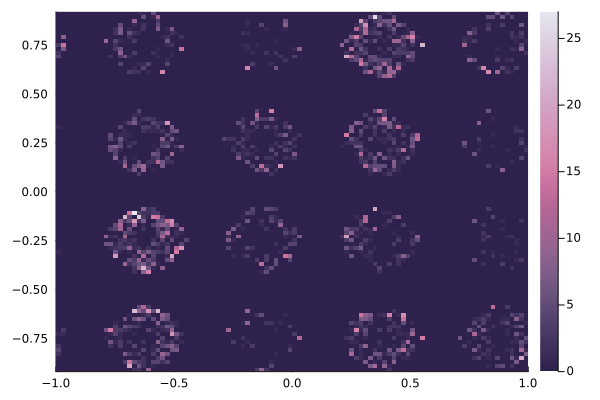
\includegraphics[width=3.5cm]{gaussian_base(1).png}
            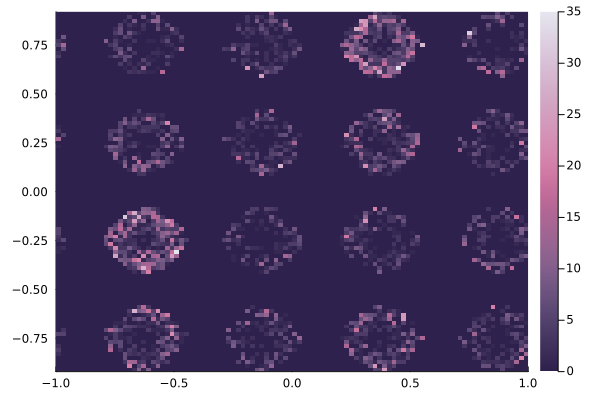
\includegraphics[width=3.5cm]{gaussian_base(2).png}
            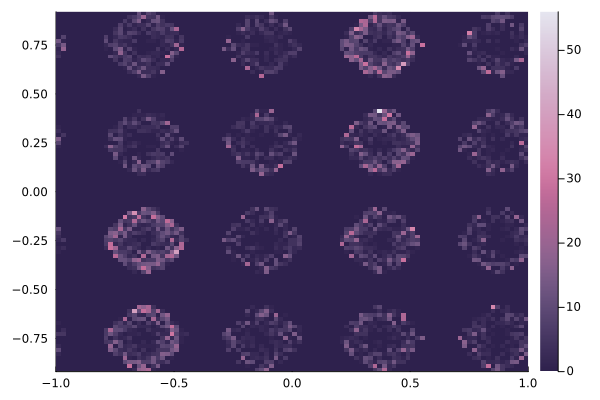
\includegraphics[width=3.5cm]{gaussian_base(3).png}
            \caption{Snapshots of accumulated samples when a wrapped Gaussian random walk base chain. The sampling is not quite even. }
            \label{fig:gaussian_rand_bc}
        \end{figure}
    \end{frame}
    \begin{frame}{The sampling results}
        \begin{figure}[h]
            \centering
            \includegraphics*[width=0.7\linewidth]{}
            \caption{}
            \label{}
        \end{figure}
        
    \end{frame}
    

\section{References}
    \begin{frame}{References}
        \bibliography{refs.bib}
    \end{frame}

\end{document}